\subsection{Zbiór "Seeds"}
    \begin{figure}[H]
        \center
        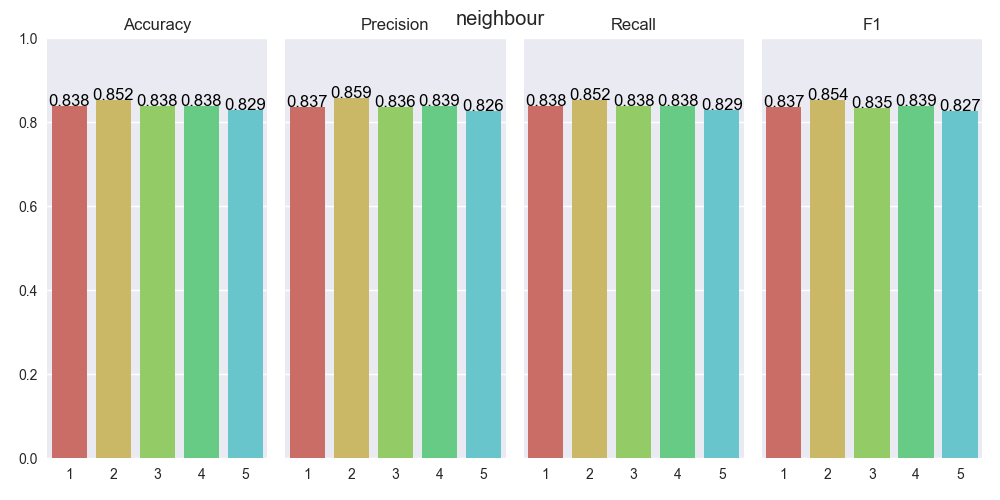
\includegraphics[width=\textwidth]{resources/plots/seeds_KFold_neighbour.png}
        \caption{Wykres wartości miar dla zbioru "Seeds" dla różnej liczby sąsiadów (kroswalidacja zwykła).}
    \end{figure}

    \begin{figure}[H]
        \center
        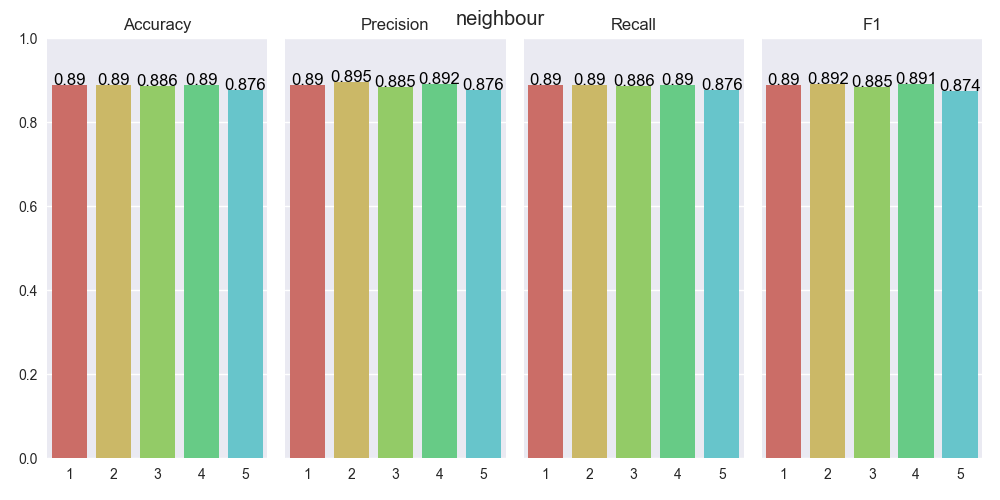
\includegraphics[width=\textwidth]{resources/plots/seeds_StratifiedKFold_neighbour.png}
        \caption{Wykres wartości miar dla zbioru "Seeds" dla różnej liczby sąsiadów (kroswalidacja stratyfikowana).}
    \end{figure}

    \pagebreak

    \begin{figure}[H]
        \center
        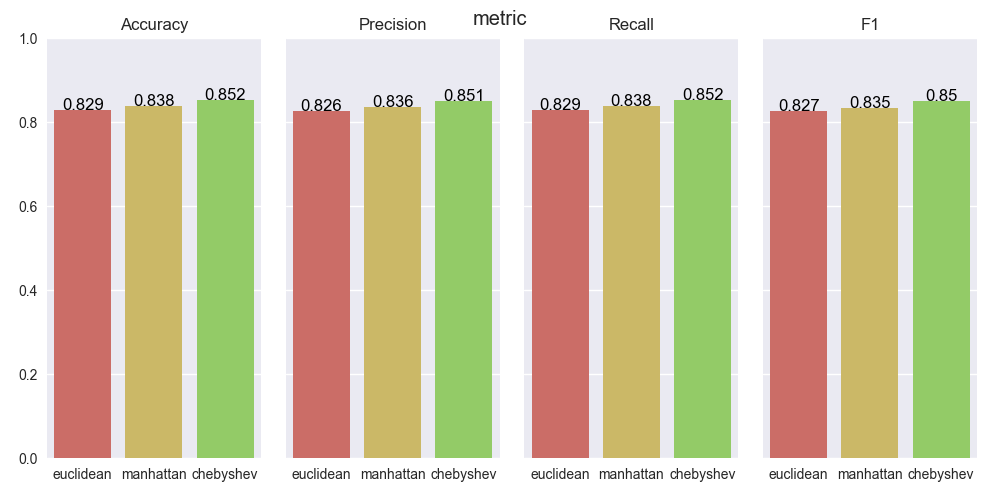
\includegraphics[width=\textwidth]{resources/plots/seeds_KFold_metric.png}
        \caption{Wykres wartości miar dla zbioru "Seeds" dla różnych metryk odległości (kroswalidacja zwykła).}
    \end{figure}

    \begin{figure}[H]
        \center
        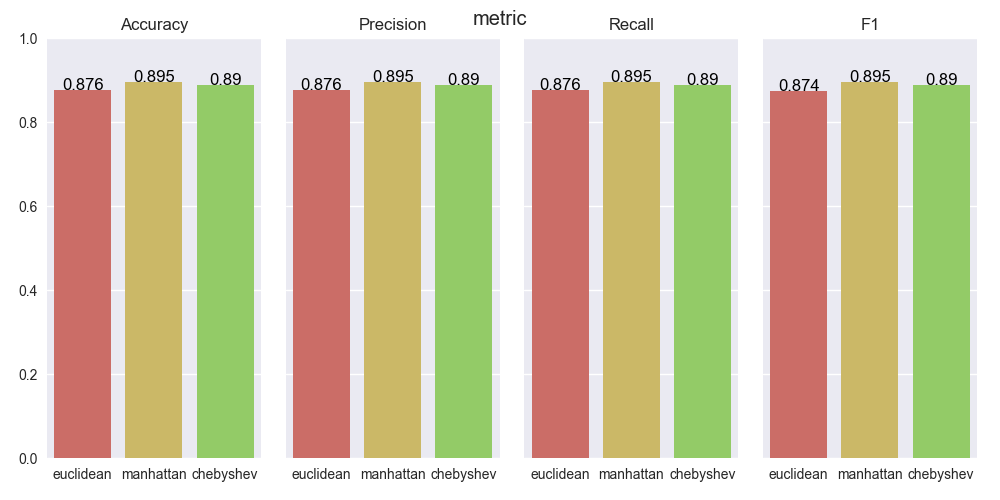
\includegraphics[width=\textwidth]{resources/plots/seeds_StratifiedKFold_metric.png}
        \caption{Wykres wartości miar dla zbioru "Seeds" dla różnych metryk odległości (kroswalidacja stratyfikowana).}
    \end{figure}

    \pagebreak

    \begin{figure}[H]
        \center
        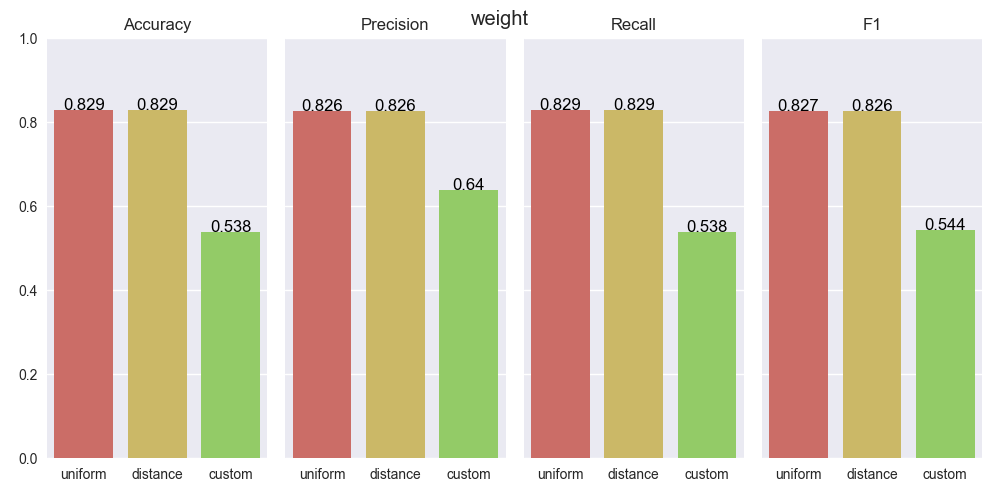
\includegraphics[width=\textwidth]{resources/plots/seeds_KFold_weight.png}
        \caption{Wykres wartości miar dla zbioru "Seeds" dla różnych sposobów głosowania (kroswalidacja zwykła).}
    \end{figure}

    \begin{figure}[H]
        \center
        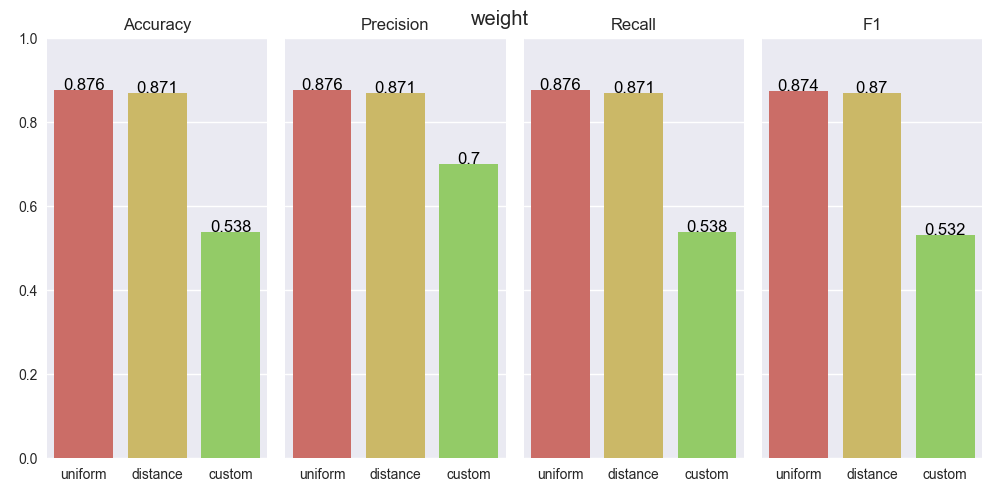
\includegraphics[width=\textwidth]{resources/plots/seeds_StratifiedKFold_weight.png}
        \caption{Wykres wartości miar dla zbioru "Seeds" dla różnych sposobów głosowania (kroswalidacja stratyfikowana).}
    \end{figure}
